\subsection{Admin UI}\label{subsec:admin-ui}
Für die übergeordnete Administrations-Oberfläche wurde auf Vorschlag des Kunden ein React-Admin Projekt erstellt.

\subsubsection{Framework Grundlagen}
React Admin ist ein Framework, spezialisiert für CRUD oberflächen.
Es setzt auf den folgenden Technologien auf:
\begin{itemize}
    \item React
    \item material UI
    \item React Router
    \item Redux
    \item Redux Saga
    \item React Final Form
\end{itemize}

Das Framework abstrahiert eine grosse Bandbreite an Funktionalität welche häufig in Administrations-Oberflächen gefordert sind.
Die Voraussetzung hierfür ist eine konsistente API welche für alle Routen dieselben Endpunkte anbieten~\cite{react-admin}.

\subsubsection{Anwendung}
Die konfigurierbaren Elemente werden jeweils in einem eigenen Component verwaltet.
React Admin unterstützt bereits Relationen zwischen diesen Komponenten.

\begin{figure}[h]
    \centering
    \label{fig:adminUi-packages}
    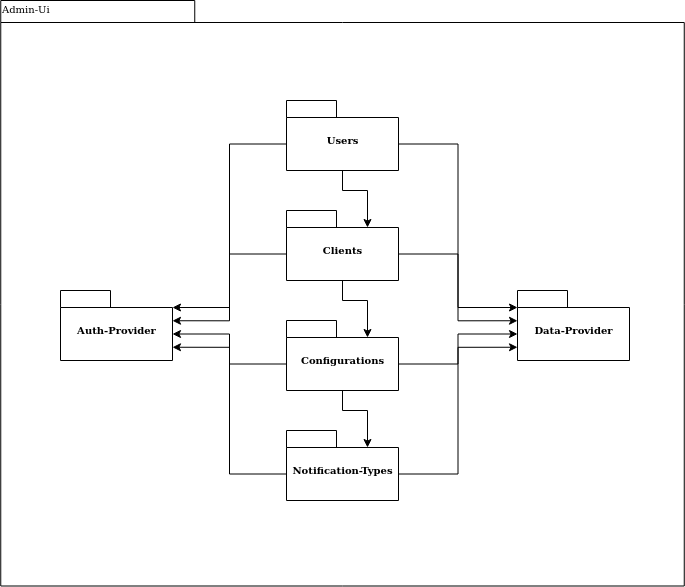
\includegraphics[width=.5\linewidth]{graphics/Admin-Ui-export}
    \caption[Admin-Ui Package Diagramm]{Admin-Ui Package Diagramm}
\end{figure}
Die Requests werden von jeweils vom Data-Provider durchgeführt der an die API des Cloudservices angepasst wird.
Vor jedem Request wird der Auth-Provider aufgerufen um zu verifizieren, dass der aktuelle Benutzer auch berechtigt ist, die gewünschte Aktion durchzuführen.

\clearpage